\documentclass[12pt, oneside]{article}

\usepackage{listings}
\usepackage[margin=0.5in]{geometry}
\usepackage{courier}
\usepackage{csvsimple}
\usepackage{graphicx}
\graphicspath{ {images/} }

\begin{document}

%titlepage
\thispagestyle{empty}
\begin{center}
\begin{minipage}{0.75\linewidth}
        \centering
        \vspace{3cm}
        {\large ECE 469\par Project 1, Part 1\par MIPS-like 32-bit ALU\par}
        \vspace{3cm}
        {\large Team ssh:\par Gregory Schmit\par Sukhbir Singh\par Phil Horwitz\par}
        \vspace{3cm}
        {\large 11 February 2018}
\end{minipage}
\end{center}
\clearpage

% testbench table

\section{Test Vector Results}
\texttt{
        \csvautotabular[respect underscore]{./alu_tvtable.csv}
}
\clearpage

% alu source code
\section{alu.sv}
\lstinputlisting[language=verilog]{./alu.sv}
\clearpage

% testvector file
\section{alu.tv}
\texttt{
        \lstinputlisting{./alu.tv}
}
\clearpage

% testbench
\section{alu\_tb.sv}
\lstinputlisting[language=verilog]{./alu_tb.sv}
\clearpage

% waveforms
\section{Waveforms}
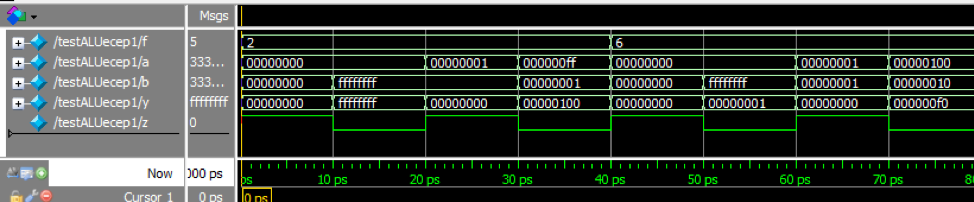
\includegraphics{alu_wf1} \newline
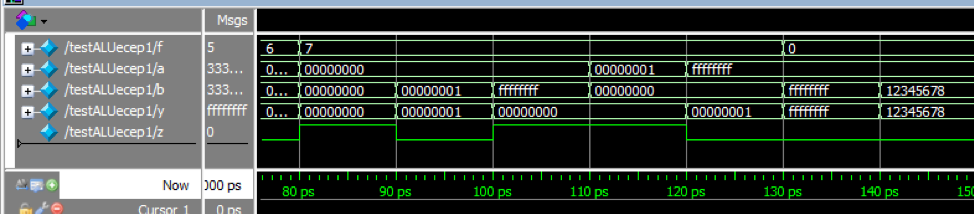
\includegraphics{alu_wf2} \newline
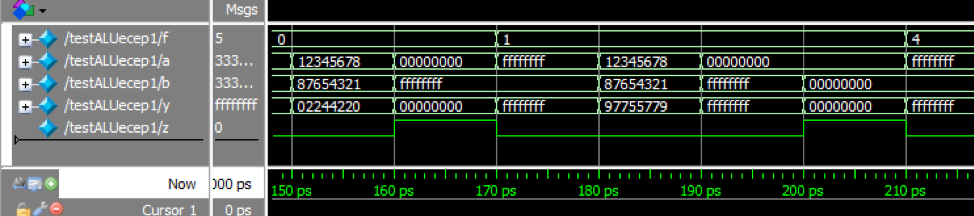
\includegraphics{alu_wf3} \newline
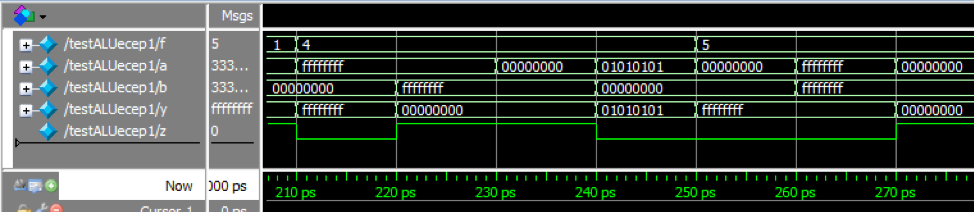
\includegraphics{alu_wf4} \newline
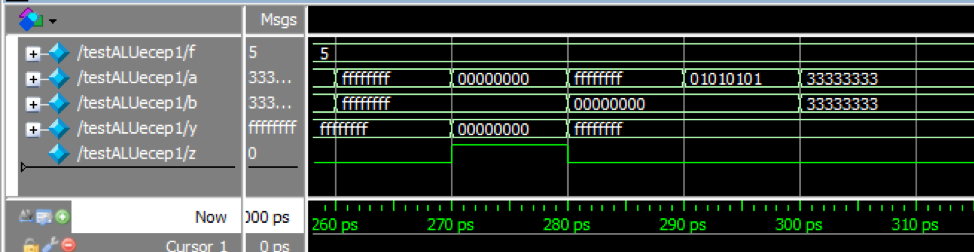
\includegraphics{alu_wf5}
\clearpage

% workload
\section{Workload Report}
The Project took between 12-16 hrs. The most time consuming part has been troubleshooting the code because of syntax errors. Also, we decided to use Latex to generate the report, so that was slightly time consuming, but should make future project reports easier to build, and easier to look at.

\end{document}
